\documentclass[a4paper,12pt]{article}
\usepackage{amsmath, amssymb}
\usepackage{xcolor}
\usepackage[most]{tcolorbox}
\usepackage{multicol}
\usepackage{geometry}
\usepackage{enumitem}
\usepackage{tasks}  % pour lister des items en colonnes
\usepackage{yhmath}
\usepackage{listing}
\usepackage{graphicx}% pour \includegraphics
\usepackage{tikz}
\usepackage{color}

\usetikzlibrary{calc,angles,quotes}
% Définition de la "pic" "tick"
\tikzset{
  pics/tick/.style args={#1}{
    code={
      % "#1" correspond à la longueur du tick.
      \draw[line width=1pt, line cap=round] (-#1/2,0) -- (#1/2,0);
    }
  }
}

\definecolor{mygreen}{rgb}{0,0.6,0}
\definecolor{mygray}{rgb}{0.5,0.5,0.5}
\definecolor{mymauve}{rgb}{0.58,0,0.82}
\definecolor{mywhite}{rgb}{0.9,0.9,0.9}

\newcommand{\footnotettfamily}{\ttfamily\footnotesize}
% \newcommand{\footnotettfamily}{\ttfamily\footnotesize}

\newcommand{\scriptttfamily}{\ttfamily\scriptsize}

\lstset{ %
  backgroundcolor=\color{mywhite},   % choose the background color
  %basicstyle=\footnotesize,        % size of fonts used for the code
  basicstyle=\ttfamily\scriptttfamily,
  breaklines=true,                 % automatic line breaking only at whitespace
  captionpos=b,                    % sets the caption-position to bottom
  commentstyle=\color{mygreen},    % comment style
escapeinside={\%*}{*)},          % if you want to add LaTeX within your code
keywordstyle=\color{blue},       % keyword style
stringstyle=\color{mymauve},     % string literal style
}

\graphicspath{ {../Images/} } % chemin vers le dossier d'images
\hyphenpenalty=1000

\geometry{left=1.5cm, right=1.5cm, top=2cm, bottom=2cm}

\tcbuselibrary{theorems}

\definecolor{PurpleEx}{HTML}{5d478b}
\definecolor{GrayEx}{HTML}{f2f2f2}
\definecolor{GrayBG}{HTML}{d9d9d9}
\definecolor{BlackSav}{HTML}{000000}
\definecolor{RedMet}{HTML}{cd5556}

\title{
\centering
\tcbset{colframe=BlackSav,colback=GrayBG}
\tcbox[tikznode]{
  Chapitre 9 \\Fonction exponentielle
}
}
\author{}
\date{}

\newtcbtheorem
[]% init options
{exercice}% name
{Exercice}% title
{%
colback=GrayEx,
colframe=PurpleEx,
fonttitle=\bfseries,
breakable=true
}% options
{ex}% prefix

\newtcbtheorem
[]% init options
{method}% name
{Méthode}% title
{%
theorem name,
colback=GrayBG,
colframe=RedMet,
fonttitle=\bfseries,
}% options
{met}% prefix

\begin{document}

\maketitle

\begin{multicols}{2}

\begin{exercice}[title=Exercice 1 $\star$ { [Calculer] }]{}{}
Simplifier, lorsque cela est possible, les expressions suivantes :
\begin{enumerate}
  \item $\exp(5)\times\exp(7)$
  \item $(\exp(5))^2$
  \item $\exp(2)+\exp(1)$
  \item $\exp(2)\times\bigl(\exp(1)\bigr)^3$
  \item $3\,\exp(2)$
  \item $\dfrac{\exp(4)\times\bigl(\exp(2)\bigr)^2}{\exp(5)}$
\end{enumerate}
\end{exercice}

\begin{exercice}[title=Exercice 2 $\star$ { [Calculer] }]{}{}
Simplifier, lorsque cela est possible, les expressions suivantes :
\begin{enumerate}
  \item $\exp(x)\times\exp(2x)$
  \item $3\bigl(\exp(x)\bigr)^2$
  \item $\exp(2x)+\exp(1)$
  \item $\bigl(\exp(x)\bigr)^3\times\bigl(\exp(-x)\bigr)^2$
  \item $4\,\exp(-x)\,\exp(5x)$
  \item $\dfrac{\exp(x)\times\bigl(\exp(3x)\bigr)^2}{\exp(8x)}$
\end{enumerate}
\end{exercice}

\begin{exercice}[title=Exercice 3 $\star$ { [Calculer] }]{}{}
Pour chacune des fonctions suivantes déterminer son ensemble de définition, son ensemble de dérivabilité et calculer $f'(x)$.
\begin{enumerate}
  \item $f : x \mapsto e^{x} + x^2 - 5$
  \item $f : x \mapsto \dfrac{e^{x}}{x-1}$
  \item $f : x \mapsto e^{3x+1}$
  \item $f : x \mapsto e^{-2x+5}$
  \item $f : x \mapsto \dfrac{x}{e^{-x+1}}$
\end{enumerate}
\end{exercice}

\begin{exercice}[title=Exercice 4 $\star$ { [Calculer] }]{}{}
Résoudre les équations suivantes :
\begin{enumerate}
  \item $e^{x-4} = e^{3x}$
  \item $e^{5x+2} = e$
  \item $e^{-3x} = 1$
  \item $e^{-3x^2} = \dfrac1e$
  \item $e^x + 1 = 0$
  \item $(x^2 - 2)\,e^{x-3} = 0$
  \item $\bigl(e^{-x+1}-1\bigr)\bigl(e^{3x}+e\bigr)=0$
  \item $-\,e^{3x} = e^{-3x}$
\end{enumerate}
\end{exercice}

\begin{exercice}[title=Exercice 5 $\star$ { [Calculer] }]{}{}
  Résoudre les inéquations suivantes :
  \begin{enumerate}
    \item $e^{x+5}\le e^{2x}$
    \item $e^{5x+2}\le 1$
    \item $e^{-3x+1}>\dfrac1{e^{-x^2}}$
    \item $\dfrac{3x-1}{e^{2x}}<0$
    \item $e^{-2x+6}\le 0$
    \item $e^{x+4}\ge \dfrac{-3}{e^{5x}}$
  \end{enumerate}
  \end{exercice}
  
  \begin{exercice}[title=Exercice 6 $\star\star\star$ { [Calculer] }]{}{}
  Résoudre les équations suivantes :
  \begin{enumerate}
    \item $e^{2x}-e^{x}=0$
    \item $2e^{2x}+2e^{x}=4$
    \item $e^{4x}+e^{2x}+1=0$
    \item $2e^{x}+4-6e^{-x}=0$
  \end{enumerate}
  \end{exercice}
  
  \begin{exercice}[title=Exercice 7 $\star\star$ { [Calculer, Raisonner] }]{}{}
  Soit $a\in\mathbb{R}$. Soit $f$ la fonction définie sur $\mathbb{R}$ par $f(x)=e^{ax}$. Montrer que $f$ est strictement croissante si, et seulement si, $a>0$.
  \end{exercice}
  
  \newcolumn

  \begin{exercice}[title=Exercice 8 $\star\star$ { [Représenter] }]{}{}
  On considère quatre fonctions $k,\ell,m,n$ définies sur $\mathbb{R}$ par :
  \[
  \begin{aligned}
  k(x)&=e^{ax}, &\ell(x)&=e^{bx},\\
  m(x)&=e^{cx}, &n(x)&=e^{dx},
  \end{aligned}
  \]
  où $a,b,c,d$ sont des réels. On donne par ailleurs les courbes représentatives de $k,\ell,m,n$ ci-dessous.  
  
  % placeholder pour le graphique  
  \begin{center}
    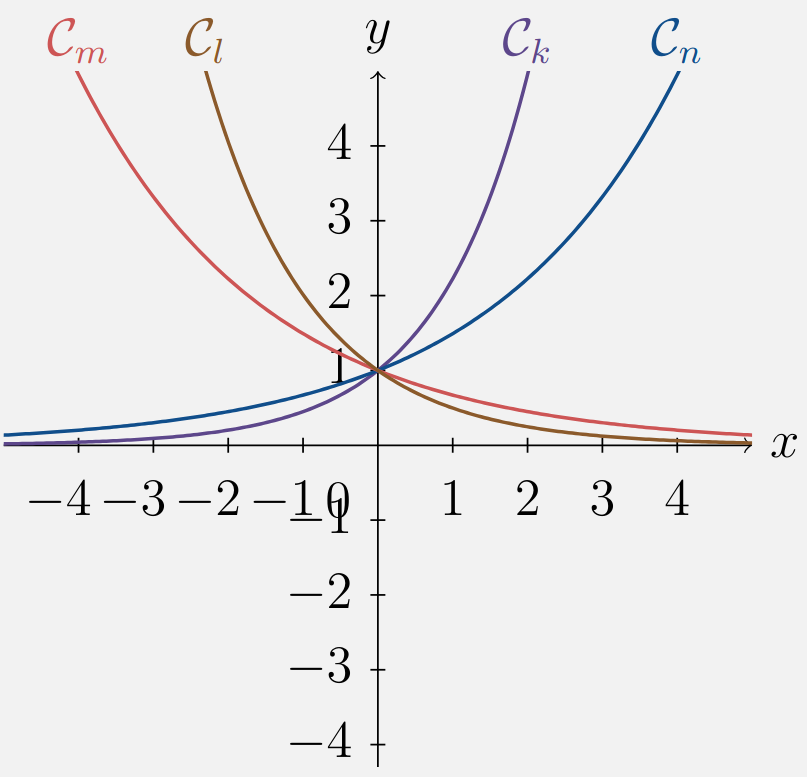
\includegraphics[width=7cm]{image.png}
  \end{center}

  
  \medskip
  \noindent
  Classer par ordre croissant les réels $a,b,c,d$.
  \end{exercice}
  
  \begin{exercice}[title=Exercice 9 $\star\star$ { [Calculer, Représenter] }]{}{}
  Étudier chacune des fonctions suivantes (parité, signe, variations) puis représenter, à main levée, sa courbe représentative :
  \begin{enumerate}
    \item $f(x)=e^x-1$
    \item $f(x)=e^{-x^2}$
    \item $f(x)=e^{3x+1}$
    \item $f(x)=(1-5x)e^x$
    \item $f(x)=(1+x)e^{-x+2}$
    \item $f(x)=(e^x)^2+5$
    \item $f(x)=(x^2-5x-1)e^{-x}$
    \item $f(x)=\dfrac{e^x}{x}$
  \end{enumerate}
  \end{exercice}
  
  \begin{exercice}[title=Exercice 10 $\star\star$ { [Représenter, Calculer] }]{}{}
    Soit $f$ la fonction définie sur $\mathbb{R}$ par 
    \[
    f(x)=e^{2x}+6e^{x}-8x-4.
    \]
    Dans le plan rapporté à un repère orthogonal, on considère :
    \begin{itemize}
      \item $C_f$ la courbe représentative de $f$ ;
      \item $D$ la droite d’équation $y=-8x-4$.
    \end{itemize}
    \begin{enumerate}
      \item Montrer que, pour tout $x\in\mathbb{R}$, $f'(x)=2(e^x-1)(e^x+4)$.
      \item Étudier le signe de $f'$ sur $\mathbb{R}$.
      \item Dresser le tableau de variations de $f$ sur $\mathbb{R}$.
      \item En déduire le signe de $f$ sur $\mathbb{R}$.
      \item La courbe $C_f$ et la droite $D$ ont-elles un point en commun ? Justifier.
    \end{enumerate}
    \end{exercice}
    
    \begin{exercice}[title=Exercice 11 $\star\star$ { [Modéliser, Calculer, Représenter] }]{}{}
    Une entreprise fabrique des pièces en acier, toutes identiques, pour l’industrie aéronautique. Ces pièces sont coulées dans des moules à la sortie du four. Elles sont stockées dans un entrepôt dont la température ambiante est maintenue à $25^\circ\mathrm{C}$. Ces pièces peuvent être modelées dès que leur température devient inférieure ou égale à $600^\circ\mathrm{C}$ et on peut les travailler tant que leur température reste supérieure ou égale à $500^\circ\mathrm{C}$.  
    
    On admet que la température, en degré Celsius, de ces pièces varie en fonction du temps. On adopte pour modèle la fonction $f$ définie sur $[0;+\infty[$ par 
    \[
    f(t)=1375\,e^{-0.075\,t}+25,
    \]
    où $t$ correspond au temps, exprimé en heures, mesuré après la sortie du four.
    \begin{enumerate}
      \item Calculer la température des pièces à la sortie du four.
      \item Étudier le sens de variation de la fonction $f$ sur l’intervalle $[0;+\infty[$. Ce résultat était-il prévisible dans le contexte de l’exercice ?
      \item Les pièces peuvent-elles être modelées 10 heures après la sortie du four ? Après 14 heures ?
      \item On souhaite déterminer le temps minimum d’attente en heures après la sortie du four avant de pouvoir modeler les pièces.
      \begin{enumerate}
        \item Compléter l’algorithme donné ci-dessous pour qu’il renvoie ce temps minimum d’attente en heure (arrondi par excès à 0,1 près).
    \begin{lstlisting}[language=Python]
from math import *
def f(t):
    return 1375*exp(-0.075*t)+25

def seuil():
    t=...
    temperature...
    while temperature > ...:
        t = t + 0.1
        temperature = ...
    return t
    \end{lstlisting}
        \item Déterminer ce temps minimum d’attente. On arrondira au dixième.
      \end{enumerate}
    \end{enumerate}
    \end{exercice}    
    
    \newpage
    \begin{exercice}[title=Exercice 12 $\star\star$ { [Modéliser, Calculer] }]{}{}
      Une entreprise pharmaceutique fabrique un soin antipelliculaire. Elle peut produire entre 200 et 2000 litres de produit par semaine. Le résultat, en dizaines de milliers d’euros, réalisé pour la production et la vente de \(x\) centaines de litres est donné par la fonction \(R\) définie sur l’intervalle \([2;20]\) par  
      \[
      R(x)=(5x-30)\,e^{-0.25x}.
      \]
      \begin{enumerate}
        \item Calculer le résultat réalisé par la fabrication et la vente de 7 centaines de litres de produit. On l’arrondira à l’euro près.
        \item Vérifier que pour la fabrication et la vente de 400 L de produit (soit \(x=4\)), l’entreprise réalise un résultat négatif (déficit).
        \item Résoudre l’inéquation \(R(x)\ge0\). Interpréter dans le contexte de l’exercice.
        \item On note \(R'\) la dérivée de \(R\). Montrer que, pour tout \(x\in[2;20]\),
        \[
          R'(x)=(-1,25\,x+12,5)\,e^{-0.25x}.
        \]
        \item En déduire la quantité de produit (en centaines de litres) que l’entreprise doit fabriquer et vendre pour obtenir le résultat maximal.
      \end{enumerate}
      \end{exercice}
      
      \newcolumn
      
      \begin{exercice}[title=Exercice 13 $\star\star$ { [Raisonner, Représenter, Calculer] }]{}{}
      \begin{enumerate}
        \item[(a)] Déterminer l’équation de la tangente à la courbe de la fonction exponentielle \(y=e^x\) au point d’abscisse \(0\).
        \item[(b)] Tracer dans un repère la courbe \(y=e^x\) et sa tangente au point d’abscisse \(0\).
        \item On considère la fonction \(f\) définie par
        \[
          f(x)=e^x - x - 1.
        \]
        \begin{enumerate}
          \item Déterminer les variations puis le signe de \(f\).
          \item En déduire que la courbe de \(y=e^x\) est toujours au-dessus de sa tangente en \(0\).
        \end{enumerate}
      \end{enumerate}
      \end{exercice}
      
      \begin{exercice}[title=Exercice 14 $\star\star\star$ { [Chercher, Raisonner, Représenter] }]{}{}
      Est-il vrai que la courbe représentative de la fonction exponentielle est située au-dessus de toutes ses tangentes ? Justifier.
      \end{exercice}
      
      \begin{exercice}[title=Exercice 15 $\star\star\star$ { [Chercher, Calculer, Représenter] }]{}{}
      On considère les fonctions  
      \[
      f\colon x\mapsto e^x
      \quad\text{et}\quad
      g\colon x\mapsto e^{-x},
      \]
      et un réel \(a\). Montrer que les tangentes respectives aux courbes \(C_f\) et \(C_g\) aux points d’abscisse \(a\) sont perpendiculaires.
      \end{exercice}
      
\end{multicols}

\end{document}
